\documentclass[11pt,a4paper]{article}

\usepackage[T1]{fontenc}
\usepackage[utf8]{inputenc}
\usepackage{lmodern}
\usepackage[a4paper,margin=2.5cm]{geometry}
\usepackage{amsmath,amssymb,amsthm}
\usepackage{bm}
\usepackage{graphicx}
\usepackage{booktabs}
\usepackage{multirow}
\usepackage{array}
\usepackage[authoryear,round]{natbib}
\usepackage{microtype}
\usepackage{setspace}
\usepackage[running]{lineno}
\usepackage{xcolor}
\usepackage{xurl}
\usepackage[colorlinks=true,linkcolor=blue!50!black,citecolor=blue!50!black,urlcolor=blue!50!black]{hyperref}
\usepackage{caption}
\captionsetup{font=small,labelfont=bf}

\newtheorem{proposition}{Proposition}
\theoremstyle{remark}
\newtheorem{remark}{Remark}

\newcommand{\meff}{m_{\mathrm{eff}}}
\newcommand{\mbar}{\bar m}
\newcommand{\E}{\mathbb{E}}
\newcommand{\Var}{\operatorname{Var}}
\newcommand{\Cov}{\operatorname{Cov}}
\newcommand{\cyd}{c\,yd$^{-3}$}

\setstretch{1.15}
\linenumbers

\title{What limits a placer drill hole? Grain counting, per-hole error and the historic Klondike drill record}

\author{Leonardo Fusar Bassini\\[4pt]
\small Dipartimento di Matematica ``Federigo Enriques'', Universit\`a degli Studi di Milano\\
\small Via Cesare Saldini 50, 20133 Milano, Italy\\
\small \href{mailto:leonardo.fusarbassini@studenti.unimi.it}{leonardo.fusarbassini@studenti.unimi.it}}

\date{}

\begin{document}

\maketitle

\begin{abstract}
\noindent
Placer gold is valued by drilling, and a single placer drill hole is notoriously unreliable: it recovers a fraction of a cubic metre of gravel holding a few gold grains. We ask how much of the scatter between holes is grain counting. Assays are modelled as a compound Poisson--gamma draw of grains from the drilled volume, with a multiplicative per-hole error, under a latent Gaussian field of log-concentration, fitted by a safeguarded Laplace approximation. The model is applied to the public drill record of the Yukon Consolidated Gold Corporation (13,358 holes, 1907--1965), after recovering unrecorded price bases and redrawn holes from the data themselves. On synthetic creeks it removes the 30\% downward bias of kriged log-grades, which the standard log-normal correction fails to fix; on Middle Dominion Creek it outperforms kriging on held-out drill lines (CRPS 1.11 against 1.21) with calibrated intervals. Yet 78 pairs of holes drilled 3--12\,m apart disagree by a typical factor of three, thirteen times the variance grain counting predicts for Dominion-like gold, and the disagreement grows with the gold in the sample, which grain counting cannot produce. The dominant term is a per-hole error with log-standard deviation 0.6--1.2. Line-spaced drilling cannot detect this error, although omitting it degrades estimates; twin holes identify it. Grain size inferred from assays alone is reliable only for large single-campaign data sets. A closed-form rule for holes per mining block follows: valley pay with fine gold needs 15--40 holes for $\pm 20\%$, lean bench ground with coarse gold several hundred.
\end{abstract}

\noindent\textbf{Keywords:} placer gold; nugget effect; compound Poisson; Gaussian process; twin holes; identifiability

\section{Introduction}

Placer gold deposits are evaluated by drilling. In the classic method, a cased churn drill advances a 6-inch pipe with a 7.5-inch shoe through frozen or thawed gravel; the material inside the shoe is bailed, panned and its gold weighed, and the gold per unit volume of ground is reported for the ``dredge section'' of gravel and broken bedrock that a dredge would dig \citep{Wells1969}. The engineering literature has long warned that a single hole is unreliable. The volume actually recovered rarely matches the theoretical shoe volume, and engineers corrected each hole by judgement; coarse gold is erratic; and a sample that holds a few grains can change its value by a factor of two with one extra particle \citep{Wells1969,Clifton1969}. Those warnings are qualitative. Modern placer evaluation, using sonic and reverse-circulation drilling, faces the same questions with the same small sample volumes.

Two quantitative traditions address the problem from different directions. Sampling theory treats the variance of a sample as a property of its particles: the Poisson argument of \citet{Clifton1969}, the sampling constants of \citet{Ingamells1973} and \citet{Ingamells1981}, and the theory of \citet{Gy1979} all predict a relative variance inversely proportional to the mass of the sample and growing with the size of the coarsest particles (with its cube, in Gy's formula). These theories are calibrated with replicate samples of the same material, which placer drill holes do not provide. Geostatistics, conversely, treats hole-to-hole scatter as the nugget of a variogram \citep{Matheron1963,Journel1978}: a single constant that absorbs every source of variation at distances shorter than the sampling interval, including grain counting, drilling error and genuinely small-scale geology. \citet{Clark2010} asked how much of a nugget is sampling error and how much is natural variability, using replicate assays; in drilling, the analogous evidence is twinned drill holes \citep{Abzalov2009}.

This paper joins the two traditions for placer drilling. We write the likelihood of a drill assay as a compound Poisson--gamma draw of grains from the drilled volume, add a multiplicative per-hole error, and embed both in a latent Gaussian field of log-concentration, in the spirit of model-based geostatistics \citep{Diggle1998,Diggle2007}. The grain-counting term has a physical signature that a constant nugget lacks: its relative variance falls as the gold in the sample rises, and it produces zero assays at a predictable rate. The per-hole term does not depend on the gold in the sample. The question is which dominates, and whether historic data can tell.

The data are the drill records of the Yukon Consolidated Gold Corporation (YCGC), which dredged the Klondike goldfields of Yukon, Canada, from 1923 to 1966. Its plans and drill logs, digitised by the Yukon Geological Survey \citep{vanLoon2016,vanLoon2017,YGS2020}, form a large public record of placer drilling. \citet{vanLoon2016,vanLoon2017} mapped parts of it and interpolated its grades; to our knowledge it has not been analysed with a statistical model of the drill measurement itself.

The contributions are as follows.
\begin{enumerate}
  \item An exact measurement model for placer drill assays with a latent spatial field, and a Laplace scheme that handles its non-log-concave likelihood; Laplace estimates agree with Markov chain Monte Carlo within 5\% at realistic grain counts (Sects.~\ref{sec:model} and \ref{sec:mcmc}).
  \item A curated version of the YCGC record, with units, unrecorded gold-price bases and redrawn holes recovered from internal evidence (Sect.~\ref{sec:data}).
  \item A decomposition of the placer drilling nugget using 78 pairs of twin holes, showing that it is dominated by a per-hole error rather than grain counting (Sect.~\ref{sec:twins}).
  \item Simple identifiability arguments, checked by simulation, that say which drilling designs can separate grain counting, per-hole error and geology (Sects.~\ref{sec:ident}, \ref{sec:simident} and \ref{sec:regional}).
  \item A reconciliation against nine dredge seasons with recorded recovery, and a closed-form rule for the number of holes a block needs (Sects.~\ref{sec:production} and \ref{sec:design}).
\end{enumerate}

\section{Data: the YCGC drill record}\label{sec:data}

\subsection{The archive}

The Yukon Geological Survey publishes the YCGC record as a public map service \citep{YGS2020} and as a downloadable geodatabase. The service holds 13,358 point records on 340 source maps (12,447 drill holes, 670 shafts and 231 bedrock test holes), 5,352 polygons of dredge cuts and thaw fields, 2,057 polygons of other workings, and an index of 933 source maps. Of the points, 8,630 carry a grade and 2,720 a bedrock elevation (Fig.~\ref{fig:overview}).

A YCGC grade is the value of gold recovered from the dredge section of a hole, in cents per cubic yard at a fixed gold price, recorded to 0.1 cent. Holes in which gold was seen but not weighable are recorded as ``trace'', digitised as 0.1\,\cyd. At \$20.67 per troy ounce, 1\,\cyd\ is 19.68\,mg of fine gold per cubic metre. Masses in this paper are fine-gold equivalents; physical grains, which carry silver, are heavier by the inverse of the fineness. Sample volumes follow from the dredge section and the 7.5-inch shoe area of 0.3068\,ft$^2$ per foot of drive \citep{Wells1969}.

\subsection{Curation}

Four problems had to be solved before the record could be modelled.

\paragraph{Units.} Thicknesses and elevations are in feet, not metres. The ratio of overburden plus dredge section to the difference between surface and bedrock elevation has median 1.08 (the dredge section includes some bedrock); 209 holes are inconsistent by more than 35\%. On Middle Dominion Creek, elevations are on a local datum.

\paragraph{Gold-price basis.} YCGC revalued some maps when the gold price changed. The price is recorded for only 14\% of holes. Three recorded values on two maps (\$1.00, \$7.60 and \$15.60) are not historical gold prices; they are ignored, and those maps are treated like others without a recorded basis. Redrawn holes resolve the question. Wherever the same hole appears on two maps, its two grades are either identical or differ by exactly the ratio of two gold prices. Among 1,982 pairs of graded holes less than 25\,m apart on different maps, 721 have identical grades, 68 differ by $35/20.67 = 1.690$ and 75 by $38.5/20.67 = 1.863$ (Fig.~\ref{fig:price}). A map whose redrawn holes consistently show one of these ratios against a map of known basis inherits the corresponding price (Appendix~\ref{app:price}). The rule confirms the two recorded revaluations it can test, and identifies two maps whose \$35 and \$38.50 bases were never recorded; left uncorrected, they would read 69--86\% too rich. Maps with no recorded or inferred basis are taken at \$20.67, and all grades are normalised to \$20.67.

\paragraph{Duplicates and non-grades.} 667 records are the same hole drawn on several maps (identical non-zero grade, less than 15\,m apart); one record per cluster is kept, preferring a record with bedrock elevation, then one with a recorded price, then the earliest map. The co-located positions of these redraws, typically 5\,m apart, measure the georeferencing error. Some layers that look like grades are not: at the same positions, thaw-field layouts on Middle Dominion read a median of 2 where the 1936 drill holes read 33\,\cyd. Layers of thaw fields, stripping, progress and workings are excluded, as are 835 grades that the digitiser marked as doubtful.

\paragraph{Releases.} The downloadable release is older than the map service (dated January 2020) and contains 2,632 fewer holes. Its shapefile stores missing values as zero, so that 3,339 of its 4,157 zero grades are unassayed holes. A model built from it would see the ground about five times more barren than the drill logs record. Where both releases contain a value, the values agree exactly, so the map service is used throughout.

After curation, 6,179 holes from 122 maps (1907--1961) carry a usable grade: a drill hole, a grade, a dredge section, an unambiguous value and no duplicate. Their median section is 14.5\,ft and their median grade 9.1\,\cyd; 6.7\% are zero.

\subsection{Study sets}

\paragraph{Middle Dominion Creek.} The 1936 drilling of Middle Dominion Creek below Lower Discovery (plan 1103) and the 1955 redraws of plans 1104--1105, checked hole by hole against the table of \citet{vanLoon2016}: 612 holes on 71 drill lines over 12.6\,km of valley, 11.8\% zero assays, one campaign with one set of conventions. One transcription error, present in both releases, was corrected to the published value.

\paragraph{Upper Sulphur Creek.} 376 holes from nine maps around the dredge No.~9 cuts of 1950--1958. Each of the nine annual cuts carries YCGC's pre-dredging estimate and the value recovered. They are the only polygons in the record with both, apart from one 1914 open cut whose ``value'' is the gold price.

\paragraph{Twin holes.} On a few maps YCGC drilled holes 3--12\,m apart: lettered infill holes (37, 37B, 37C, \dots) and whole check lines drilled beside earlier lines. Section~\ref{sec:twins} uses every such pair.

\paragraph{Campaigns.} The 33 maps with at least 60 usable grades (62--393 holes each) are treated as separate drilling campaigns in Sect.~\ref{sec:regional}.

\begin{figure}[t]
  \centering
  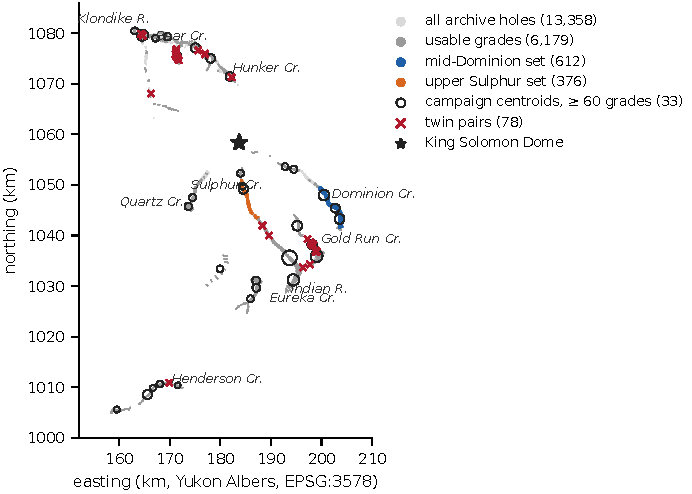
\includegraphics[width=\textwidth]{figures/fig1_overview.pdf}
  \caption{The YCGC drill record in the Klondike goldfields. Grey: archive holes and holes with usable grades. Coloured: the Middle Dominion and upper Sulphur study sets. Circles: centroids of the 33 campaigns with at least 60 usable grades. Crosses: twin pairs. Star: King Solomon Dome, the inferred lode source of most Klondike placer gold \citep{Lowey2006}.}
  \label{fig:overview}
\end{figure}

\begin{figure}[t]
  \centering
  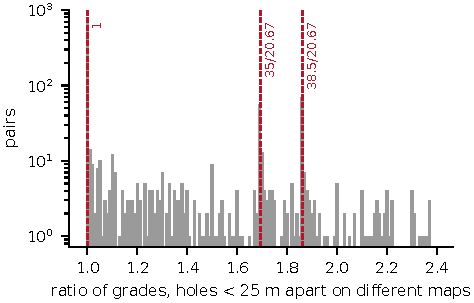
\includegraphics[width=0.62\textwidth]{figures/fig2_price_ratios.pdf}
  \caption{Ratio of grades for graded holes less than 25\,m apart on different maps. Peaks sit exactly at 1 (redrawn holes) and at the ratios of the gold prices \$35 and \$38.50 to \$20.67 (revalued redraws), which identifies unrecorded price bases.}
  \label{fig:price}
\end{figure}

\section{Model}\label{sec:model}

\subsection{Grain counting}

Let $c(x)$ be the concentration of gold in the ground at position $x$ (mg\,m$^{-3}$) and $V$ the volume of a drill sample. The sample holds a random number of grains,
\begin{equation}\label{eq:cpg}
N \sim \mathrm{Poisson}(\lambda),\quad \lambda = \frac{cV}{\mbar},\qquad
m_k \overset{\mathrm{iid}}{\sim} \mathrm{Gamma}\!\left(\alpha,\ \theta = \mbar/\alpha\right),\qquad
S = \sum_{k=1}^{N} m_k,\qquad G = S/V,
\end{equation}
where $\mbar$ is the number-weighted mean grain mass and $\alpha$ the shape of the grain-mass distribution. By the law of total variance, $\E[S] = cV$ and $\Var[S] = \lambda\,\E[m^2] = cV\meff$, with
\begin{equation}\label{eq:meff}
\meff = \frac{\E[m^2]}{\E[m]} = \left(1 + \frac{1}{\alpha}\right)\mbar,
\qquad
\mathrm{CV}^2(G) = \frac{\meff}{cV},
\qquad
P(G = 0) = e^{-cV/\mbar}.
\end{equation}
The effective grain mass $\meff$ is the mass-weighted mean grain mass and is dominated by the coarse fraction. Equation~\eqref{eq:meff} generalises the Poisson argument of \citet{Clifton1969}, in which relative error falls as $X^{-1/2}$ for $X$ equal grains, to unequal grains. Unlike a Tweedie model \citep{Jorgensen1987,Dunn2005,Anderson2025}, in which the grain distribution is tied to the mean so that $\Var[S] \propto \E[S]^p$ with $1 < p < 2$, here the grain distribution is a property of the gold and $\Var[S] \propto \E[S]$.

For an observed mass $s > 0$ the likelihood is the Poisson mixture
\begin{equation}\label{eq:lik}
p(s \mid \lambda) = \sum_{n \ge 1} \frac{e^{-\lambda}\lambda^n}{n!}\,
\frac{s^{n\alpha - 1} e^{-s/\theta}}{\Gamma(n\alpha)\,\theta^{n\alpha}},
\end{equation}
a zero has probability $e^{-\lambda}$, and a trace assay is the censored event $0 < S < s_{\mathrm{tr}}$, with the gamma distribution function in place of the density and $s_{\mathrm{tr}}$ the mass of 0.15\,\cyd\ in the sample. Differentiating in $\eta = \log\lambda$,
\begin{equation}\label{eq:score}
\frac{\partial \log p}{\partial \eta} = \E[N \mid \mathrm{obs}] - \lambda,
\qquad
\frac{\partial^2 \log p}{\partial \eta^2} = \Var[N \mid \mathrm{obs}] - \lambda,
\end{equation}
so that inference needs only the posterior distribution of the unseen grain count (Appendix~\ref{app:lik}). The sum in \eqref{eq:lik} is evaluated over a window of $\pm 12$ posterior standard deviations around its mode. The second derivative in \eqref{eq:score} can be positive: the likelihood is not log-concave in $\eta$ when $\alpha$ is small.

Because $\lambda$ depends on $V/\mbar$, an error in the assumed sample volume is absorbed by $\mbar$; inferred grain masses are relative to the 7.5-inch shoe volume. The ratio $\meff/\mbar = 1 + 1/\alpha$ does not depend on the volume.

\subsection{Per-hole error}

A drill hole is not only a grain draw. The volume recovered differs from the theoretical shoe volume through caving, packing and boulders; engineers corrected each hole by judgement, with upward corrections of up to a factor of two \citep{Wells1969}; and a hole that catches a crevice at the bedrock surface samples different gravel from one 5\,m away. All of these multiply the concentration seen by one hole and not its neighbour. We write
\begin{equation}\label{eq:perhole}
\log\lambda_i = f(x_i) + \log V_i - \log\mbar + e_i,\qquad e_i \overset{\mathrm{iid}}{\sim} N(0, \sigma_h^2),
\end{equation}
with $f = \log c$. The per-hole factor $e^{e_i}$ has median one, so $f$ is a median. Whether the extra gold is real (small-scale geology) or the factor is a measurement error with mean one, the mean concentration of a block is $\exp(f + \sigma_h^2/2)$, which is 28\% above the median field for $\sigma_h = 0.7$. Only a factor biased high on average, such as sloughing of gravel into the casing, would need no correction.

\subsection{Latent field in valley coordinates}

Placer pay follows the valley. Each hole receives coordinates $(s, n)$: $s$ is the distance along a valley axis and $n$ the signed offset across it, positive towards the left limit. Neither the axis nor, on some maps, the drill lines are recorded. Both are reconstructed from the holes alone (Appendix~\ref{app:frame}). On Middle Dominion the reconstructed lines reproduce the labels of plan 1103 exactly (adjusted Rand index 1.0; \citealp{Hubert1985}).

The log-concentration is a Gaussian process,
\begin{equation}\label{eq:gp}
f \sim \mathcal{GP}\big(\beta_0,\ k\big),\qquad
k(x, x') = \sigma^2 (1 + \sqrt{3}\,r)\,e^{-\sqrt{3}\,r},\qquad
r = \sqrt{(\Delta s/\ell_s)^2 + (\Delta n/\ell_n)^2},
\end{equation}
an anisotropic Mat\'ern-3/2 covariance \citep{Stein1999} with separate length scales along and across the valley. 

\subsection{Inference}

Let $u_i = f(x_i) + e_i$ be the latent log-concentration seen by hole $i$, so that $\bm u \sim N(\beta_0\bm 1, \Sigma)$ with $\Sigma = K + \sigma_h^2 I$, and $\log\lambda_i = u_i + \log V_i - \log\mbar$. Derivatives of the log-likelihood with respect to $u_i$ are those of \eqref{eq:score}. For fixed hyperparameters $\psi = (\beta_0, \sigma, \ell_s, \ell_n, \mbar, \alpha, \sigma_h)$, the posterior mode $\hat{\bm u}$ is found by Newton's method \citep[Alg.~3.1]{Rasmussen2006}, with two modifications. The negative Hessian of the log-likelihood, which can be negative by \eqref{eq:score}, is replaced by the positive weight $W_i = \max(\lambda_i - \Var[N_i \mid \mathrm{obs}],\ \epsilon)$, and each Newton step is followed by a backtracking line search. Non-log-concave likelihoods make the unmodified Newton iteration fragile, as discussed for the Student-$t$ likelihood by \citet{Jylanki2011}. The Laplace approximation to the marginal likelihood \citep{Tierney1986,Williams1998},
\begin{equation}\label{eq:laplace}
\log Z(\psi) \approx \sum_i \log p(y_i \mid \hat u_i) - \tfrac{1}{2}\,\hat{\bm a}^\top(\hat{\bm u} - \beta_0\bm 1) - \sum_i \log L_{ii},\qquad
LL^\top = I + W^{1/2} \Sigma W^{1/2},
\end{equation}
with $\hat{\bm a} = \Sigma^{-1}(\hat{\bm u} - \beta_0\bm 1)$, is maximised over $\psi$ by L-BFGS-B \citep{Byrd1995} on transformed parameters, warm-starting each mode search from the previous one. Predictions of $f$ at new locations use the standard Gaussian formulas with $W$ \citep{Rasmussen2006}, and predictive assays are obtained by sampling $f$, the per-hole error and the grain draw \eqref{eq:cpg}. Section~\ref{sec:mcmc} checks the approximation against Markov chain Monte Carlo.

\subsection{What identifies each component}\label{sec:ident}

Three components produce scatter between holes: grain counting, the per-hole error and the field. Their signatures differ, but not always in ways a given drilling design can see. The following observation is elementary, but it decides what historic data can show.

\begin{proposition}[Per-hole error and short-range geology]\label{prop:confound}
Let $n$ holes be at least $d$ apart and let a component of $f$ have covariance $\tau^2\rho(\|x - x'\|/\ell)$ with $\rho(0) = 1$ and $\rho(u) \to 0$ as $u \to \infty$. On the design, its covariance matrix is $\tau^2(I + E)$ with $\|E\|_2 \le (n - 1)\,\sup_{u \ge d/\ell} |\rho(u)|$. As $\ell/d \to 0$ it becomes indistinguishable from a per-hole error with $\sigma_h^2 = \tau^2$.
\end{proposition}

\begin{proof}
The diagonal of the covariance matrix is $\tau^2$. Each off-diagonal entry is bounded in absolute value by $\tau^2 \sup_{u \ge d/\ell}|\rho(u)|$, and since $E$ is symmetric, Gershgorin's theorem bounds $\|E\|_2$ by its largest absolute row sum. The likelihood depends on the latent covariance only through its values on the design.
\end{proof}

YCGC holes are 40--60\,m apart on a line and lines 100--200\,m apart, so any geology varying on a scale of metres is, for this data, a per-hole error. Twin holes reduce $d$ and break the equivalence.

Grain counting is separated from both by its dependence on the gold in the sample. For a hole with known concentration $c$, the Fisher information on grain size arrives through two channels (Appendix~\ref{app:fisher}). The zero/non-zero indicator carries
\begin{equation}\label{eq:izero}
I_{\mathrm{zero}}(\log\mbar) = \frac{\lambda^2 e^{-\lambda}}{1 - e^{-\lambda}},
\end{equation}
which peaks at $\lambda \approx 1.6$ grains per sample and is negligible once samples hold more than about ten grains. The spread of positive assays, in a Gaussian approximation on the log scale with non-grain variance $v_0$ (per-hole error and unresolved geology), carries
\begin{equation}\label{eq:idisp}
I_{\mathrm{disp}}(\log\meff) \approx \frac{1}{2}\left(\frac{x/(1+x)}{v_0 + \log(1 + x)}\right)^2,\qquad x = \frac{\meff}{cV},
\end{equation}
which vanishes when the grain variance $x$ is small next to $v_0$. Thick, rich sections therefore say almost nothing about grain size, and thin, lean sections say a great deal. Both expressions assume $c$ known and are upper bounds on what real assays carry.

\subsection{Precision of a block estimate}\label{sec:blockrule}

Consider $n$ holes in a block of uniform concentration $c$. Each assay is $c$ times a per-hole factor of mean one and relative variance $h^2 = e^{\sigma_h^2} - 1$, times a grain-counting factor of mean one and relative variance $g^2 = \meff/(cV)$. The two are independent, so each assay has relative variance $\kappa^2 = (1 + h^2)(1 + g^2) - 1$, and by the delta method
\begin{equation}\label{eq:kappa}
\Var\!\left[\log\frac{\bar G}{c}\right] \approx \frac{\kappa^2}{n},
\qquad
\kappa^2 = \left(1 + h^2\right)\left(1 + \frac{\meff}{cV}\right) - 1.
\end{equation}
Two consequences follow. Grain counting contributes more than the per-hole error only while a sample holds less gold than
\begin{equation}\label{eq:crossover}
(cV)^\ast = \frac{\meff}{h^2},
\end{equation}
and the number of holes needed for a relative precision $s$ is $n \approx \kappa^2/s^2$. Variation of $c$ within the block adds to $\kappa^2$, so these counts are lower bounds.

\section{Validation design}\label{sec:validation}

Random hold-out leaks information: holes on one line are tens of metres apart. All validation is spatial \citep{Roberts2017}. \emph{Leave-lines-out}: drill lines are split into ten groups and each group is predicted from the others, which tests interpolation between drilled lines. \emph{Blocks}: the valley is cut into 1\,km segments, each predicted from holes more than 150\,m away, which tests extrapolation. Predictions are scored by the continuous ranked probability score (CRPS; \citealp{Gneiting2007}) of $\log(1 + G)$ with $G$ in mg\,m$^{-3}$, coverage of 90\% predictive intervals, Spearman correlation, and the share of total gold accumulation (grade times section) in the 20\% of held-out holes ranked highest. On synthetic data, where the field is known, predictions of $\log c$ are scored directly.

The comparison methods work on $\log(1 + G)$: ordinary kriging with anisotropy from directional variograms, the classical geostatistical approach, and a Gaussian process with Gaussian likelihood and the covariance \eqref{eq:gp}. For predictions of $\log c$, the kriging variance is reduced by the nugget.

\section{Simulation studies}\label{sec:sim}

\subsection{Benchmark}\label{sec:benchmark}

Synthetic creeks reproduce the YCGC design: a sinuous 9\,km valley, drill lines every 150\,m with holes every 40\,m across a 600\,m floor. The pay channel has a Gaussian cross-profile (standard deviation 35\,m) offset towards the left limit and meandering with a 1.8\,km wavelength; its richness varies along the channel with a 600\,m correlation length. The log-concentration is $4.0 + (3.5 + r(s))\,\phi(n)$, with $r$ the richness and $\phi$ the cross-profile. Dredge sections are log-normal (median 8\,ft) and grains follow \eqref{eq:cpg} with $\mbar = 1$\,mg and $\alpha = 0.6$ ($\meff = 2.7$\,mg). Grades are recorded to 0.1\,\cyd\ with traces as in the archive. A creek has 720 holes, a median of five grains per sample, 2.8\% zeros and 2.6\% traces. The valley frame is built through the midpoints of the drill lines, as for real data.

\begin{table}[t]
\centering
\small
\caption{Synthetic benchmark: prediction of the true $\log c$ at held-out drill lines. Mean $\pm$ standard deviation over three independent creeks. ``+ nugget/2'' and ``+ noise/2'': standard log-normal correction of the kriged or GP log-grade by half the fitted nugget or white-noise variance.}
\label{tab:synthetic}
\setlength{\tabcolsep}{2.2pt}
\begin{tabular}{lcccccc}
\toprule
method & RMSE & bias & CRPS & 90\% cov. & top-20\% gold & $\rho$ in channel \\
\midrule
kriging, log-grade & $0.848 \pm 0.015$ & $-0.34 \pm 0.01$ & $0.508 \pm 0.019$ & 0.97 & 0.70 & $0.31 \pm 0.02$ \\
kriging + nugget/2 & $0.832 \pm 0.037$ & $-0.27 \pm 0.13$ & $0.501 \pm 0.031$ & 0.98 & 0.69 & $0.28 \pm 0.06$ \\
GP, log-grade & $0.837 \pm 0.012$ & $-0.32 \pm 0.00$ & $0.460 \pm 0.006$ & 0.91 & 0.68 & $0.33 \pm 0.06$ \\
GP + noise/2 & $0.798 \pm 0.042$ & $0.19 \pm 0.12$ & $0.453 \pm 0.027$ & 0.92 & 0.68 & $0.32 \pm 0.07$ \\
grain counting & $\mathbf{0.719 \pm 0.004}$ & $\mathbf{-0.10 \pm 0.04}$ & $\mathbf{0.411 \pm 0.003}$ & 0.96 & 0.69 & $0.35 \pm 0.08$ \\
\bottomrule
\end{tabular}
\end{table}

Kriging and the Gaussian process on log-grades underestimate the concentration by about 30\% ($-0.34$ and $-0.32$ in $\log c$; Table~\ref{tab:synthetic}, Fig.~\ref{fig:synthetic}). With a few grains per sample, the logarithm of an assay is biased low, both by Jensen's inequality and through zeros. The standard remedy adds half the nugget variance to the kriged log-grade, which is exact when the measurement error is log-normal with mean one. It does not work here. The variograms fitted at a 40\,m hole spacing have little or no nugget, so the correction barely moves kriging ($-0.27$). The Gaussian process, whose white-noise variance is 0.75--1.06, is over-corrected ($+0.19$), because grain-counting noise on the log scale is skewed, not Gaussian. The grain-counting field removes most of the bias without any correction, and its RMSE is 15\% below that of kriging and 10\% below that of the best corrected baseline. The ranking of rich ground is the same for all three methods. Over 1\,km held-out blocks no method extrapolates the meandering channel: the correlation within the channel is 0.03--0.05 for every method. Claims about ground far from drilling must come from geology, not interpolation. In this low-count setting the grain mass is underestimated two- to threefold ($\meff$ 0.8--1.2\,mg against 2.7\,mg), although the field itself is recovered (see Sect.~\ref{sec:discussion}).

\begin{figure}[t]
  \centering
  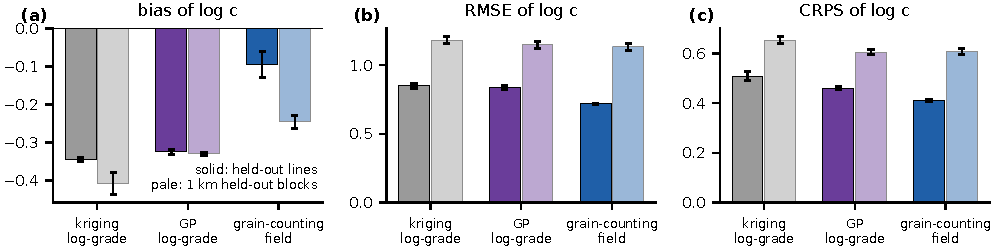
\includegraphics[width=\textwidth]{figures/fig3_synthetic.pdf}
  \caption{Synthetic benchmark, three creeks. (a) Bias, (b) RMSE and (c) CRPS of the predicted $\log c$ at held-out drill lines (solid) and held-out 1\,km blocks (pale). Error bars: standard deviation over creeks.}
  \label{fig:synthetic}
\end{figure}

\subsection{Identifiability}\label{sec:simident}

The same generator, on a 4.5\,km valley (355 holes) with Dominion-like grains ($\mbar = 3.85$\,mg, $\alpha = 0.58$, $\meff = 10.5$\,mg), tests Proposition~\ref{prop:confound}. Each hole's concentration is multiplied by a per-hole factor with $\sigma_h = 0$ or $0.8$, and the creek is drilled either on lines alone or with a twin 8\,m from 15\% of the holes. Both models are fitted to three creeks per scenario (Table~\ref{tab:ident}, Fig.~\ref{fig:ident}).

\begin{table}[t]
\centering
\small
\caption{Identifiability study (three creeks per row). $\Delta\log Z$: marginal likelihood of the model with a per-hole term minus that of grains only. True $\meff = 10.5$\,mg.}
\label{tab:ident}
\begin{tabular}{cllcccc}
\toprule
true $\sigma_h$ & design & model & $\meff$ (mg) & $\hat\sigma_h$ & $\Delta\log Z$ & RMSE of $f$ \\
\midrule
0 & lines & grains only & $8.2 \pm 0.9$ & -- & \multirow{2}{*}{0.0} & 0.62 \\
0 & lines & grains + per-hole & $8.2 \pm 0.9$ & 0.08 & & 0.62 \\
0 & lines + twins & grains only & $9.4 \pm 0.6$ & -- & \multirow{2}{*}{0.1} & 0.59 \\
0 & lines + twins & grains + per-hole & $9.2 \pm 0.5$ & 0.15 & & 0.59 \\
0.8 & lines & grains only & $8.4 \pm 3.3$ & -- & \multirow{2}{*}{0.4} & 0.83 \\
0.8 & lines & grains + per-hole & $8.1 \pm 3.1$ & 0.58 & & 0.70 \\
0.8 & lines + twins & grains only & $11.3 \pm 1.9$ & -- & \multirow{2}{*}{8.2} & 0.80 \\
0.8 & lines + twins & grains + per-hole & $8.1 \pm 0.1$ & 0.68 & & 0.68 \\
\bottomrule
\end{tabular}
\end{table}

Three results stand out. First, line-spaced drilling cannot detect a real per-hole error: with $\sigma_h = 0.8$ the marginal likelihood improves by only 0.4 when the term is added. Leaving the term out nonetheless worsens the estimate of the field by 18\% (RMSE 0.83 against 0.70); absence of evidence in the marginal likelihood is not evidence of absence. Second, twins identify the term ($\Delta\log Z = 8.2$) and stabilise the grain mass, whose spread across creeks falls from 3.1 to 0.1\,mg. Third, without a per-hole term the grain mass absorbs whatever scatter it can: it is erratic on lines alone and biased upwards once twins expose the scatter. Apart from that biased case, all estimates are 10--23\% below the true $\meff$; Section~\ref{sec:mcmc} shows that this is not an artefact of the Laplace approximation.

\begin{figure}[t]
  \centering
  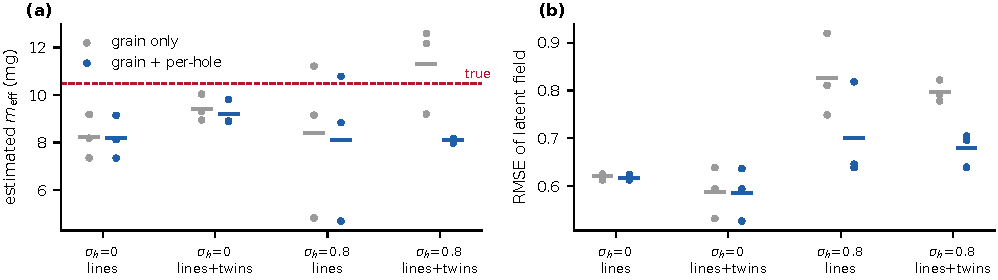
\includegraphics[width=\textwidth]{figures/fig6_identifiability.pdf}
  \caption{Identifiability study. (a) Estimated effective grain mass and (b) RMSE of the latent field, for each creek (dots) and their mean (bars), by true per-hole error, design and fitted model. Dashed line: true $\meff$.}
  \label{fig:ident}
\end{figure}

\section{Results on the Klondike record}\label{sec:results}

\subsection{Middle Dominion Creek}\label{sec:dominion}

On the 612 Middle Dominion holes, the model selected by marginal likelihood is grain counting with the field (Table~\ref{tab:dominion}); neither a per-hole term nor a probability of structural zeros (barren holes) is supported. The field has correlation lengths of 130\,m along and 33\,m across the valley, consistent with the pay channel of about 45\,m width mapped by \citet{vanLoon2016}. The effective grain mass is 10.5\,mg ($\mbar = 3.85$\,mg, $\alpha = 0.58$). Independent observations describe Dominion gold as flat, rounded and well travelled, with flaky grains up to about 3\,mm in lower Dominion \citep{Froese2001,Chapman2010}. An effective mass of 10\,mg corresponds to a flake about 1.5\,mm across and 0.3\,mm thick, within that range.

\begin{table}[t]
\centering
\small
\caption{Middle Dominion Creek, 612 holes. Fitted parameters and held-out scores. Leave-lines-out (LOLO): ten groups of drill lines; blocks: 1\,km held-out segments.}
\label{tab:dominion}
\begin{tabular}{lcccc}
\toprule
\multicolumn{5}{l}{\emph{Model selection}} \\
model & $\log Z$ & $\ell_s$, $\ell_n$ (m) & $\meff$ (mg) & other \\
\midrule
grains + field & $-2775.0$ & 130, 33 & 10.5 & -- \\
+ per-hole error & $-2775.0$ & 130, 33 & 10.5 & $\hat\sigma_h = 0.003$ \\
+ structural zeros, $\pi_0 = 0.01$ & $-2785.8$ & 146, 33 & 11.5 & -- \\
+ structural zeros, $\pi_0 = 0.1$ & $-2808.2$ & 131, 32 & 10.8 & -- \\
per-hole error fixed at $\sigma_h = 0.7$ & $-2778.6$ & 214, 49 & 10.3 & -- \\
\midrule
\multicolumn{5}{l}{\emph{Held-out scores}} \\
method & CRPS & Spearman & 90\% coverage & gold in top 20\% \\
\midrule
kriging, LOLO & 1.210 & 0.34 & 0.88 & 27.8\% \\
GP, LOLO & 1.189 & 0.32 & 0.86 & 32.1\% \\
grain-counting field, LOLO & \textbf{1.115} & \textbf{0.38} & \textbf{0.915} & \textbf{34.9\%} \\
grain-counting field, $\sigma_h = 0.7$, LOLO & 1.107 & 0.38 & 0.913 & 34.1\% \\
kriging, blocks & 1.301 & 0.06 & 0.87 & 25.5\% \\
GP, blocks & 1.279 & $-0.02$ & 0.85 & 25.0\% \\
grain-counting field, blocks & \textbf{1.190} & \textbf{0.13} & \textbf{0.913} & \textbf{27.9\%} \\
\bottomrule
\end{tabular}
\end{table}

On held-out drill lines the grain-counting field scores better than kriging and the Gaussian process on every measure, and its 90\% intervals are calibrated (0.915) where theirs are too narrow (0.88 and 0.86). Ranking held-out ground by the model puts 34.9\% of its gold in the top fifth, against 27.8\% for kriging. Over 1\,km held-out blocks all methods are close to chance, as on synthetic creeks.

Because line-spaced drilling cannot see a per-hole error (Sect.~\ref{sec:simident}), its absence here is not evidence that there is none. Forcing $\sigma_h = 0.7$, the value suggested by the twin holes of Sect.~\ref{sec:twins}, costs 3.5 log-units of marginal likelihood. It leaves the grain mass unchanged and the held-out scores unchanged or slightly better, and lengthens the correlation scales: the per-hole error trades against the field, not against grain mass. A profile over $\sigma_h$ confirms this: $\meff$ is 10.5, 10.0, 10.0 and 10.5\,mg at $\sigma_h = 0$, 0.3, 0.6 and 0.8, and falls to 8.4 and 6.1\,mg only at 1.0 and 1.2. Structural zeros (a probability $\pi_0$ that a hole is barren whatever the concentration) do not change the grain mass either: on a profile over $\pi_0$, $\log Z$ is largest at $\pi_0 = 0$ and $\meff$ stays between 10.3 and 11.5\,mg up to $\pi_0 = 0.1$. At $\pi_0 = 0.1$, the solution with fine gold ($\meff = 2.3$\,mg) lies 9.4 log-units below the coarse one. The likelihood of a zero assay becomes flat in $\lambda$ once $\pi_0 > 0$, which the Laplace approximation handles less well, so these comparisons are approximate; the drop of 10.7 log-units between $\pi_0 = 0$ and 0.01 is larger than the model change warrants and reflects that loss of accuracy. Target probabilities on unmined ground under $\sigma_h = 0$ and $\sigma_h = 0.7$ have rank correlation 0.94.

The fitted field reproduces where YCGC mined (Fig.~\ref{fig:dominion}). The company's dredge cuts and thaw fields cover 45\% of the drilled valley floor but contain 78\% of the drill-indicated gold.

\begin{figure}[t]
  \centering
  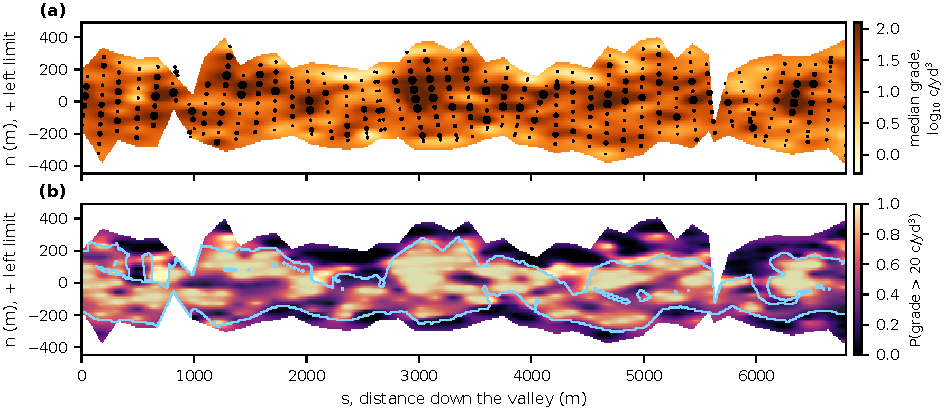
\includegraphics[width=\textwidth]{figures/fig4_dominion.pdf}
  \caption{Middle Dominion Creek, first 6.8\,km of the reconstructed valley. (a) Median predicted grade ($\log_{10}$\,\cyd\ at \$20.67) with the 1936 drill holes (dot size proportional to grade). (b) Probability that the grade exceeds 20\,\cyd; YCGC dredge cuts and thaw fields are outlined and shaded.}
  \label{fig:dominion}
\end{figure}

\subsection{Twin holes}\label{sec:twins}

Among 706 pairs of holes with a dredge section less than 12\,m apart, 85 lie on the same map. Removing five pairs that are double records of one hole (same grade and section) and six with the same hole number leaves 78 twin pairs on 13 maps, a median of 8.3\,m apart: 38 on Bear Creek (1912), 15 on Gold Run (1941), 9 on lower Hunker and 16 on ten other maps. In 72 pairs both holes contain gold. Distances between twins are measured on one map, so the georeferencing error between maps (about 5\,m) does not affect them. Most pairs come from lettered infill holes and from check lines drilled beside earlier lines, rather than from re-drilling of single holes with suspicious results. There is no clear offset between the two drilling series on a map: the median log-ratio between series is $-0.09$ on lower Hunker (4 of 9 pairs positive) and $+0.56$ on Gold Run (7 of 10; sign test $p = 0.34$).

\begin{table}[t]
\centering
\small
\caption{Twin holes 3--12\,m apart: robust variance $(1.4826\,\mathrm{MAD})^2$ of $\log(G_1/G_2)$ for the 72 pairs with gold in both holes, overall and by tercile of the gold in the sample, against twins simulated at the same volumes and levels.}
\label{tab:twins}
\begin{tabular}{lcccc}
\toprule
 & all pairs & \multicolumn{3}{c}{tercile of gold per sample} \\
 & & 6--88\,mg & 88--181\,mg & 181--1259\,mg \\
\midrule
observed & \textbf{2.87} & 0.58 & 2.45 & 5.14 \\
simulated: grains only, $\meff = 10$\,mg & 0.23 & 0.81 & 0.22 & 0.09 \\
simulated: grains only, $\meff = 90$\,mg & 1.59 & 3.99 & 2.27 & 0.86 \\
simulated: 10\,mg grains + per-hole $\sigma_h = 0.8$ & 1.69 & 2.17 & 1.67 & 1.39 \\
\bottomrule
\end{tabular}
\end{table}

Twins disagree by a median factor of 3.06 ($|\log(G_1/G_2)| = 1.12$). The robust variance of the log-ratio, 2.87, is about thirteen times what grain counting with Dominion-like gold predicts (Table~\ref{tab:twins}, Fig.~\ref{fig:twins}). Because the pairs cluster by map, uncertainty is assessed by resampling whole maps (Table~\ref{tab:twinci}). The ratio to Dominion-like grain counting is 12.7 (90\% interval 3.7--23.5), and 11.4 (2.2--27.6) without the 35 Bear Creek pairs. On size alone, however, very coarse gold cannot be excluded: the ratio to grain counting with $\meff = 90$\,mg is 1.8 (0.6--2.9).

The shape of the disagreement is what rules grain counting out. Grain-count disagreement must fall as the gold in the sample rises, from 0.81 to 0.09 across the terciles for 10\,mg gold; the observed disagreement rises instead, from 0.58 to 5.14. In a regression of $\log|\log(G_1/G_2)|$ on the log of the gold per sample with a fixed effect for each map, grain counting alone gives a negative slope at every grain mass from 10 to 300\,mg: simulated means lie between $-0.51$ and $-0.38$, and the 95th percentiles are at most $+0.04$. The observed slope is $+0.26$ (90\% interval $-0.04$ to 0.60), and the association is positive within maps (permutation of gold content within maps, $p = 0.045$). Without Bear Creek the slope is $+0.17$ ($-0.13$ to 0.88), still above the 95th percentile of every grain-only simulation. Rich ground is erratic at the scale of metres.

\begin{table}[t]
\centering
\footnotesize
\caption{Twin holes, uncertainty from resampling whole maps (2,000 cluster-bootstrap samples; 90\% intervals). Ratio: observed robust variance of $\log(G_1/G_2)$ over that of twins simulated with grains only. Slope: regression of $\log|\log(G_1/G_2)|$ on log gold per sample with map fixed effects; grain counting alone gives $-0.51$ to $-0.38$. $p$: within-map permutation test of a positive association.}
\label{tab:twinci}
\setlength{\tabcolsep}{3pt}
\begin{tabular}{lcccccc}
\toprule
pairs & $n$ (maps) & robust var. & ratio, 10\,mg & ratio, 90\,mg & slope & $p$ \\
\midrule
gold in both holes & 72 (11) & 2.87 (0.97--4.34) & 12.7 (3.7--23.5) & 1.8 (0.6--2.9) & 0.26 ($-0.04$--0.60) & 0.045 \\
without Bear Creek & 37 (10) & 2.20 (0.62--4.54) & 11.4 (2.2--27.6) & 1.4 (0.4--3.2) & 0.17 ($-0.13$--0.88) & 0.12 \\
without old workings & 61 (11) & 2.59 (0.97--4.33) & 13.7 (4.0--24.7) & 1.8 (0.6--3.0) & 0.30 ($-0.03$--0.60) & 0.09 \\
\bottomrule
\end{tabular}
\end{table}

The full latent model confirms this. On the four maps with at least four twin pairs, adding the per-hole term raises the marginal likelihood on every one, by 1.7, 2.2, 9.0 and 15.7 log-units, with $\hat\sigma_h$ between 0.62 and 1.23 (Fig.~\ref{fig:twins}b). Without the term, the model imitates the per-hole scatter on three of the four maps with implausibly short cross-valley correlation lengths of 5--14\,m; with it, these lengthen to 16--934\,m. The grain-mass estimates move substantially (Gold Run: 88 to 45\,mg; lower Hunker: 59 to 4.5\,mg).

The hole-to-hole nugget of this churn drilling is therefore dominated by a multiplicative per-hole error of a factor of two to three ($\sigma_h \approx 0.6$--1.2). By Proposition~\ref{prop:confound}, it cannot be divided further with these data into drilling error and geology at scales below 3--12\,m. Its growth with the gold in the sample points to geology: rich gravel concentrates gold in bedrock crevices and riffles that one hole catches and another misses. Grain counting is a floor that matters where samples hold little gold.

\begin{figure}[t]
  \centering
  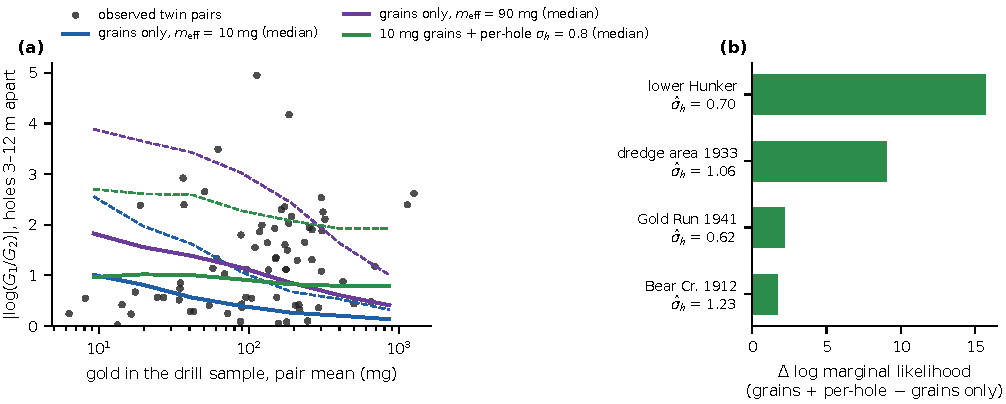
\includegraphics[width=\textwidth]{figures/fig5_twins.pdf}
  \caption{Twin holes. (a) Absolute log-ratio of grades for pairs 3--12\,m apart against the gold in the sample, with the median (solid) and 90th percentile (dashed) of simulated twins under three nugget models. (b) Gain in marginal likelihood from a per-hole error term on the four maps with at least four twin pairs, with the fitted $\hat\sigma_h$.}
  \label{fig:twins}
\end{figure}

\subsection{Grain mass across 33 campaigns}\label{sec:regional}

If grain size could be read from assays, the record would yield a map of it, to be set against the systematic changes of Klondike gold particles with distance of transport from their lode sources \citep{Knight1994,Knight1999}. We fitted the model separately to each of the 33 campaigns with at least 60 usable grades, in coordinates aligned with the principal axes of each campaign's holes, and profiled the marginal likelihood over $\mbar$ on a grid from 0.1 to 100\,mg, refitting all other parameters at each point.

The likelihood is confident. Across the grid the profiles fall by 17--285 log-units, and 29 of the 33 have a closed 95\% interval. The depth of each profile tracks the zero-channel information \eqref{eq:izero} summed over the campaign's holes (Spearman $\rho = 0.78$; Fig.~\ref{fig:profiles}b).

The answers, however, do not agree. The best-fitting $\mbar$ ranges from 0.1 to 10\,mg between campaigns on the same creek (six Dominion campaigns span the whole range). It tracks the median dredge section ($\rho = -0.49$, $p = 0.004$) and the share of zero assays ($\rho = +0.54$, $p = 0.001$), not the distance from King Solomon Dome ($\rho = -0.09$, $p = 0.62$; Fig.~\ref{fig:profiles}a). On single campaigns the estimate also depends on the model. On a Dominion campaign of 149 holes (map 26222), allowing structural zeros and a per-hole error lowers $\meff$ from 20\,mg to 1.4\,mg and raises $\log Z$ by 1.6: ``coarse gold'' and ``fine gold plus barren holes plus per-hole error'' fit about equally well. On the largest Sulphur campaign (393 holes, map 26681), a per-hole error alone lowers $\meff$ from 40\,mg to 3.5\,mg and raises $\log Z$ by 17.

Middle Dominion, with 612 holes from one campaign, is the exception (Sect.~\ref{sec:dominion}). So are the three upper-Sulphur bench campaigns, whose thin sections and many zeros give them high information: their estimates (29--84\,mg) are stable under a per-hole error and structural zeros, and agree with descriptions of coarse, angular gold up to several grams in upper Sulphur \citep{vanLoon2017}. In general, however, grain size can be read from the assays only from large single-campaign data sets, after checking the alternatives that mimic coarse gold: barren ground, per-hole error and a heavier grain-size tail. A regional map of grain size from the historic assays is not supportable. The sharp profiles illustrate a general hazard: a confident likelihood does not identify a quantity when the model omits a component that produces the same data.

\begin{figure}[t]
  \centering
  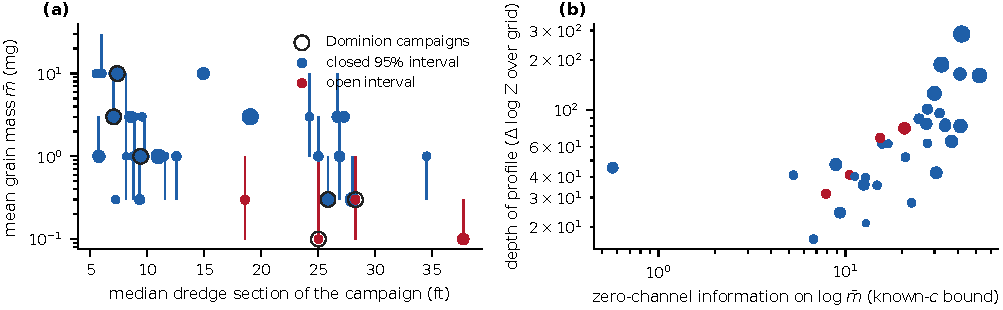
\includegraphics[width=\textwidth]{figures/fig7_profiles.pdf}
  \caption{Grain mass across 33 campaigns. (a) Best-fitting mean grain mass and 95\% profile interval on the grid, against the median dredge section; blue: closed interval, red: open; ringed: Dominion campaigns; dot size proportional to the number of holes. (b) Depth of each profile against the zero-channel information of its holes \eqref{eq:izero}, computed at the observed grades with $\mbar = 3$\,mg.}
  \label{fig:profiles}
\end{figure}

\subsection{Reconciliation with production}\label{sec:production}

The nine dredge No.~9 seasons on upper Sulphur Creek (1950--1958) each record YCGC's estimate before dredging and the value recovered, at \$20.67, for 0.39--0.61 million cubic yards per season. YCGC's estimates had no season-to-season skill (Pearson $r = 0.06$ with the recovered grade). Over the nine seasons the dredge recovered 23\% more value than estimated, from 9\% more gravel. Recovered grades span only 17--38\,\cyd, so with nine blocks no estimator can show ranking skill.

\begin{table}[t]
\centering
\small
\caption{Upper Sulphur Creek, nine dredge seasons: RMSE of log(estimated/recovered grade) and total bias. Sensitivity runs change only the radius used to reconstruct drill lines, or value two disputed maps at \$35 instead of \$20.67.}
\label{tab:sulphur}
\begin{tabular}{lccc}
\toprule
estimator & primary & line radius 40\,m & disputed maps at \$35 \\
\midrule
YCGC recorded estimate & 0.37; $-12\%$ & 0.37; $-12\%$ & 0.37; $-12\%$ \\
mean of holes in the block & 0.64; $+74\%$ & 0.64; $+74\%$ & 0.62; $+70\%$ \\
kriging, block held out & 0.65; $+75\%$ & 1.09; $-48\%$ & 0.43; $-10\%$ \\
grain-counting field, block held out & 0.62; $+70\%$ & 0.42; $+29\%$ & 0.56; $+55\%$ \\
\bottomrule
\end{tabular}
\end{table}

Model block grades are the mean predicted concentration, $\exp(\mu + s^2/2)$ with $\mu$ and $s^2$ the latent mean and variance, over a 5\,m grid covering each cut; for kriging, the same log-normal back-transform is applied with the nugget excluded. Each season is predicted with the holes inside its cut removed. No model beats YCGC's own estimate (Table~\ref{tab:sulphur}, Fig.~\ref{fig:sulphur}a). YCGC's block estimates are about half the raw mean of the holes inside the blocks, so the company applied a weighting or deduction that the public record does not document, and dredge recovery is not recorded. A model of gold in the ground 30--70\% above the gold recovered is consistent with recoveries of 60--80\%. Absolute block grades also move by tens of percent with defensible analysis choices: changing only the radius used to reconstruct drill lines moves kriging from $+75\%$ to $-48\%$, and the disputed price basis of two maps moves it again. The grain-counting field is more stable but still spans $+29\%$ to $+70\%$. At block scale the dominant uncertainty lies in conventions, not in the interpolator.

How large should the error of a drill-based block estimate be? Simulating from each fitted model the true block grade together with the mean of the assays at the actual hole positions and sections, the predicted log-error spread is 0.90 (robust 0.64) for the upper Sulphur seasons, of which 0.29 is spatial, and 0.44 for the 19 Middle Dominion dredge years. The ordering agrees with the evidence: the observed spread of the mean of holes against recovery is 0.45 (robust 0.29) on Sulphur, and \citet{vanLoon2016} reports block errors on Middle Dominion that imply a spread of at least 0.18--0.20. The size does not: on Sulphur, the grains-only model predicts twice the observed error. Scanning $\meff$ with everything else fixed, the observed robust spread is best matched by $\meff \lesssim 10$\,mg, but its 90\% bootstrap interval (0.08--0.80) admits any $\meff$ between 0.3 and about 100\,mg (Fig.~\ref{fig:sulphur}b). Nine blocks cannot measure grain size.

\begin{figure}[t]
  \centering
  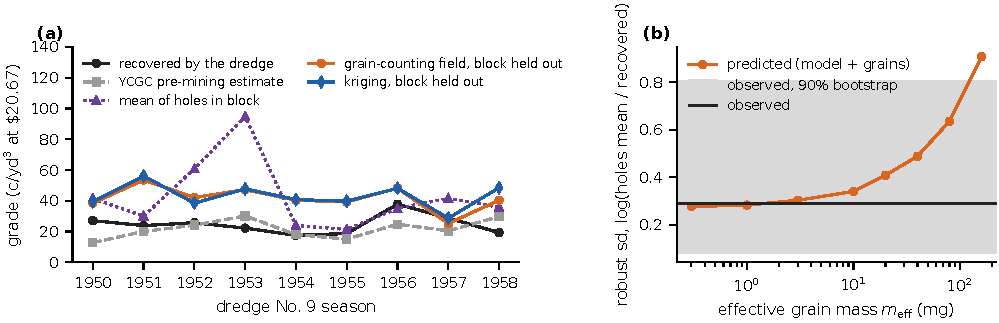
\includegraphics[width=\textwidth]{figures/fig8_sulphur.pdf}
  \caption{Upper Sulphur Creek. (a) Grade recovered by dredge No.~9 in each season against YCGC's estimate, the mean of the holes in the block, and the two models with the block held out. (b) Predicted spread of log(mean of holes / true block grade) as a function of the effective grain mass, against the observed spread and its 90\% bootstrap interval.}
  \label{fig:sulphur}
\end{figure}

\subsection{Holes per block}\label{sec:design}

Monte Carlo simulation with exact grain draws and a per-hole factor of mean one checks \eqref{eq:kappa}. For $n \ge 16$ holes and samples holding at least one effective grain mass of gold, the simulated variance is 0.79--1.02 times the formula, which therefore errs on the safe side. Where samples hold less gold than one effective grain mass, the ratio ranges from 0.69 to 2.05; the formula can then be optimistic by up to a factor of two, and more for fewer holes. The crossover \eqref{eq:crossover} lies at about 16\,mg of gold per sample for Dominion-like gold ($\meff = 10$\,mg, $\sigma_h = 0.7$) and at about 80\,mg for coarse gold ($\meff = 50$\,mg). The twin pairs hold a median of about 140\,mg of gold, on the per-hole side of the crossover, which is why their disagreement does not fall with the gold in the sample.

\begin{table}[t]
\centering
\small
\caption{Holes per block for a relative precision of $\pm 20\%$ and $\pm 30\%$ (one standard deviation), from \eqref{eq:kappa}, for $\sigma_h$ between 0.6 and 0.9. Grain share: fraction of the per-hole relative variance due to grain counting. The counts are lower bounds: variation of grade within the block adds to them.}
\label{tab:design}
\setlength{\tabcolsep}{4pt}
\begin{tabular}{lcccc}
\toprule
ground (grade, section, $\meff$) & gold/sample & grain share & $\pm 20\%$ & $\pm 30\%$ \\
\midrule
Dominion valley pay (20\,\cyd, 20\,ft, 10\,mg) & 68\,mg & 0.25--0.10 & 17--40 & 8--18 \\
Dominion lean ground (5\,\cyd, 20\,ft, 10\,mg) & 17\,mg & 0.57--0.32 & 32--65 & 15--29 \\
Gold Run pay (34\,\cyd, 15\,ft, 45\,mg) & 87\,mg & 0.54--0.29 & 30--61 & 14--27 \\
Sulphur bench, rich (20\,\cyd, 7\,ft, 50\,mg) & 24\,mg & 0.83--0.63 & 86--149 & 39--67 \\
Sulphur bench, lean (5\,\cyd, 7\,ft, 50\,mg) & 6\,mg & 0.95--0.87 & 311--501 & 138--223 \\
\bottomrule
\end{tabular}
\end{table}

On valley-bottom pay with fine gold, 15--40 holes per block give $\pm 20\%$, and the per-hole error, not grain counting, sets the number (Table~\ref{tab:design}, Fig.~\ref{fig:design}). Lean bench ground with coarse gold needs several hundred holes per block; no practical drilling density values it to $\pm 20\%$. This is the regime in which placer engineers have always turned to bulk sampling \citep{Wells1969}; Equation~\eqref{eq:kappa} attaches a number to the advice.

\begin{figure}[t]
  \centering
  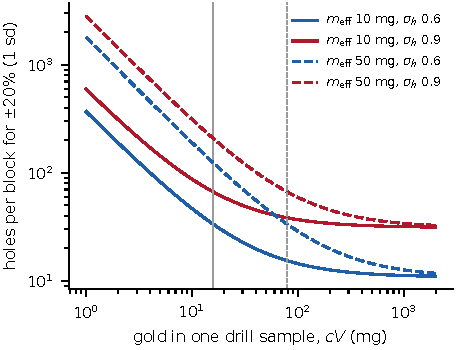
\includegraphics[width=0.62\textwidth]{figures/fig9_design.pdf}
  \caption{Holes per block for $\pm 20\%$ (one standard deviation) against the gold in one drill sample, from \eqref{eq:kappa}. Solid: $\meff = 10$\,mg; dashed: 50\,mg. Grey lines: crossover \eqref{eq:crossover} for $\sigma_h = 0.7$.}
  \label{fig:design}
\end{figure}

\subsection{Is the Laplace approximation adequate?}\label{sec:mcmc}

With the spatial hyperparameters fixed at their fitted values, the latent field was sampled by elliptical slice sampling \citep{Murray2010}, which needs no tuning, and $(\beta_0, \log\mbar, \log\alpha)$ by random-walk Metropolis, with flat priors on the fitting ranges. Chains of 20,000 iterations were run, keeping the last 14,000.

\begin{table}[t]
\centering
\small
\caption{Effective grain mass: Laplace estimate against the conditional posterior by MCMC.}
\label{tab:mcmc}
\begin{tabular}{lccc}
\toprule
case & Laplace & MCMC median (90\% int.) & truth \\
\midrule
synthetic, Dominion-like grains (355 holes) & 9.2\,mg & 9.4 (7.5--12.0)\,mg & 10.5\,mg \\
Middle Dominion (612 holes) & 10.5\,mg & 10.3 (8.9--11.8)\,mg & -- \\
\bottomrule
\end{tabular}
\end{table}

On both, the Laplace estimate agrees with the posterior median to within 3\%, and on the synthetic creek the posterior interval covers the true value (Table~\ref{tab:mcmc}). The shortfall of Sect.~\ref{sec:simident} is therefore not caused by the approximation; it is within posterior uncertainty for a single creek, and its consistent sign suggests the field prior, since the synthetic channel is not a Gaussian process.

Mixing is slow: the effective sample size for $\meff$ is below 20 over the 14,000 kept iterations of a chain started at the mode. To check convergence on Middle Dominion, a second chain was started far from the mode, with the field at its prior mean and the grain mass tripled. It reached the region of the first chain after about 15,000 iterations. Over the last 3,500 iterations of both chains the Gelman--Rubin statistic for $\log\meff$ is 1.04, the medians are 9.9 and 10.2\,mg, and the pooled posterior is 10.0\,mg (8.8--11.4), within 5\% of the Laplace estimate. Chains of 6,000 iterations started at the mode had not yet left its neighbourhood, so short runs would have overstated agreement.

\section{Discussion}\label{sec:discussion}

\paragraph{What limits a placer drill hole.} The twin holes rank the sources of error. First comes a per-hole error of a factor of two to three, which no amount of gold in the sample reduces and which, if anything, grows in rich ground. Second, at block scale, come the conventions that turn hole values into reserves: the estimation factor and the recovery, which on upper Sulphur shift block grades by tens of percent. Grain counting comes third. It matters only below the crossover \eqref{eq:crossover}, in thin and lean sections with coarse gold, where it dominates completely. Sampling theory in the tradition of \citet{Gy1979} and \citet{Clifton1969} is therefore necessary but not sufficient for placer drilling: it describes the floor, not the scatter. On a hard-rock tin deposit, \citet{Clark2010} reached the analogous conclusion with replicate assays: sampling and assay error were a small part of the nugget.

\paragraph{Using historic drilling.} The latent grain-counting field interpolates between drilled lines better than kriging, with calibrated uncertainty, and the ground it ranks highest is the ground YCGC mined. It does not forecast block grades better than the company's own estimates, and absolute grades depend on undocumented conventions. Historic placer drilling can rank and locate ground relative to the drilling; turning it into tonnes and grams requires a local calibration against production, of which a modern test pit is the most direct.

\paragraph{Designing new drilling.} Two recommendations follow. Twin 10--15\% of holes: it is the only way to measure the per-hole error, which limits block estimates and cannot be seen otherwise (Proposition~\ref{prop:confound}, Table~\ref{tab:ident}). And plan hole numbers per block with \eqref{eq:kappa}, using the twins for $\sigma_h$ and either grain-size analyses or a pilot campaign for $\meff$. \citet{Abzalov2009} recommends 20--30 twinned holes where local variability is high. Our results put a scale on that advice for placers, and show that the twins also correct the grain-size estimate.

\paragraph{Limitations.} Most twin pairs come from four maps, and the pairs are close (3--12\,m) but not coincident. Half of the pairs with gold in both holes are from the 1912 Bear Creek map; without them the excess over Dominion-like grain counting remains (11-fold, 90\% interval 2--28), but the trend with gold content is not significant on its own ($p = 0.12$). We do not know why YCGC drilled each pair, and re-drilling of holes with surprising results would inflate the disagreement. Whether fine, travelled gold such as Dominion's has a smaller per-hole error cannot be tested directly, because Dominion has no twins. The grain-mass distribution is modelled as a gamma; a heavier tail would raise $\meff$ relative to $\mbar$ and is one of the alternatives that mimic coarse gold (Sect.~\ref{sec:regional}). The valley frame is reconstructed from the holes and becomes unreliable where a valley folds back on itself within a few drill-line spacings. The MCMC check fixes the spatial hyperparameters and covers Dominion-like grain counts. In the low-count benchmark, where the grain mass is underestimated two- to threefold, a chain of 11,000 iterations had not converged, so it remains open whether the approximation or the field prior is responsible. Finally, the record contains only nine blocks with recorded recovery, too few to measure block-level error with useful precision.

\section{Conclusions}

A placer drill hole is limited less by the few grains it contains than by a multiplicative error of a factor of two to three that belongs to the hole: to its volume, its correction and the metre-scale geology it happens to intersect. Grain counting sets a floor that matters only when samples hold little gold. Line-spaced drilling cannot see the per-hole error, although ignoring it degrades estimates; twin holes reveal it. With an exact grain-counting likelihood and a latent spatial field, historic drilling becomes a calibrated tool for ranking ground. A simple rule, $\Var[\log \bar G/c] \approx \kappa^2/n$, then says how many holes a block needs and when no drilling density will do.

\section*{Acknowledgements}
The Yukon Geological Survey digitised and published the YCGC records under the Open Government Licence -- Yukon. Contains information licensed under the Open Government Licence -- Yukon.

\section*{Declarations}

\paragraph{Funding.} No funding was received for this work.

\paragraph{Competing interests.} The author has no competing interests to declare.

\paragraph{Data availability.} The YCGC drill record is published by the Yukon Geological Survey at \url{https://deptweb.gov.yk.ca/prod/rest/services/YGS_HistoricPlacer/Historic_placer_data/MapServer}. The curated data set derived from it is available with the code.

\paragraph{Code availability.} The code that reproduces every number, table and figure is available at \url{https://github.com/Maths1723/Klondyke_Project}. A script in the repository recomputes every number printed in this paper from the analysis outputs and checks it against the text.

\appendix

\section{Likelihood evaluation}\label{app:lik}

Write $\eta = \log\lambda$ and $\theta = \mbar/\alpha$. For an observed mass $s > 0$, the joint probability of $n$ grains and mass $s$ is
\[
q_n = \frac{e^{-\lambda}\lambda^n}{n!}\,\frac{s^{n\alpha - 1}e^{-s/\theta}}{\Gamma(n\alpha)\,\theta^{n\alpha}},\qquad n \ge 1,
\]
and $p(s \mid \lambda) = \sum_n q_n$. Since $\partial \log q_n/\partial\eta = n - \lambda$,
\[
\frac{\partial \log p}{\partial \eta} = \sum_n \frac{q_n}{p}(n - \lambda) = \E[N \mid s] - \lambda,
\qquad
\frac{\partial^2 \log p}{\partial \eta^2} = \Var[N \mid s] - \lambda,
\]
the second from differentiating the first with $\partial \E[N \mid s]/\partial\eta = \Var[N \mid s]$. The same identities hold for a trace observation, with $q_n$ containing the gamma distribution function $P(n\alpha, s_{\mathrm{tr}}/\theta)$ in place of the density, and for a zero, for which $N = 0$ with certainty and the derivatives are $-\lambda$ and $-\lambda$. Hence $\partial^2\log p/\partial\eta^2 > 0$ whenever the posterior of $N$ is over-dispersed relative to Poisson, which happens when $\alpha$ is small and $s$ is compatible with very different grain counts.

The terms $\log q_n$ are concave in $n$ for fixed $s$, so the sum is concentrated around the mode $n^\ast$, which solves
\[
\eta + \alpha\log(s/\theta) = \psi(n + 1) + \alpha\,\psi(n\alpha),
\]
with $\psi$ the digamma function; the root is found by bisection. The sum is evaluated in log-space over $n^\ast \pm (12\,\mathrm{sd} + 10)$, with the posterior standard deviation sd from the local curvature, and is capped at 6,000 terms per hole. Numerically, the probabilities of zero, trace and positive outcomes sum to one within $10^{-6}$, and the analytic derivatives agree with finite differences.

\section{Gold-price basis}\label{app:price}

For each pair of holes less than 25\,m apart on different maps, both graded above 0.5\,\cyd, the ratio of the higher grade to the lower is compared with the price ratios $35/20.67$, $35.3/20.67$ and $38.5/20.67$. A pair matches a ratio if it agrees to within 0.6\%, or to within one recording unit (0.1\,\cyd) of the rescaled lower grade. Matches are counted for each combination of richer map, reference map and price. Where at least three pairs match and the reference map has a known \$20.67 basis, the richer map is assigned that price; a map whose inferred price differs from a recorded one is flagged as a conflict. The rule confirms the recorded bases of maps 26344 (\$35, 38 pairs) and 26345 (\$38.50, 61 pairs), and assigns previously unrecorded bases to maps 25097 (\$35, 14 pairs) and 26343 (\$38.50, 16 pairs). One conflict remains: maps 26683 and 26743 on upper Sulphur share 84 holes with identical grades, although 26743 records \$35 and 26683 records nothing. YCGC valued the 1950--1958 seasons at \$20.67, so both maps are taken at \$20.67 in the primary analysis and at \$35 in a sensitivity run (Table~\ref{tab:sulphur}).

\section{Valley frame and drill lines}\label{app:frame}

The valley axis is first estimated as a principal curve of the hole positions \citep{Hastie1989}: starting from the first principal axis, the holes are projected onto the current curve, the median position of the holes is taken in 200\,m bins along it, and a smoothing spline is refitted. Drill lines are then the connected components of a graph that links holes less than a radius $R$ apart. YCGC lines cross the valley with holes about 60\,m apart, and lines are 100--200\,m apart, so a radius between the two separates them. The axis is refitted through the midpoints of lines with at least three holes, and the two steps are repeated three times. On Middle Dominion, $R = 70$\,m. Elsewhere, $R$ is 1.15 times the 75th percentile of the nearest-neighbour distance, clipped to 40--90\,m. Each hole is then assigned its arc length $s$ along the axis and its signed perpendicular offset $n$.

\section{Fisher information on grain size}\label{app:fisher}

\paragraph{Zero channel.} Let $Z = \mathbb{1}\{S = 0\}$, with $P(Z = 1) = p = e^{-\lambda}$ and $\lambda = cV/\mbar$, so that $\partial p/\partial\log\mbar = \lambda e^{-\lambda}$. For a Bernoulli variable, $I = (\partial p/\partial\phi)^2/\{p(1 - p)\}$, which gives
\[
I_{\mathrm{zero}}(\log\mbar) = \frac{\lambda^2 e^{-2\lambda}}{e^{-\lambda}(1 - e^{-\lambda})} = \frac{\lambda^2 e^{-\lambda}}{1 - e^{-\lambda}}.
\]
It tends to zero as $\lambda \to 0$ (almost every sample is empty) and as $\lambda \to \infty$ (none is), and is maximal at $\lambda \approx 1.59$, where it equals 0.65.

\paragraph{Dispersion channel.} If the log-assay is approximately Gaussian with variance $v = v_0 + \log(1 + x)$, $x = \meff/(cV)$, the information on a variance parameter $\phi$ is $I = \tfrac12(\partial v/\partial\phi)^2/v^2$. With $\phi = \log\meff$, $\partial v/\partial\phi = x/(1 + x)$, which gives \eqref{eq:idisp}. The expression vanishes as $x \to 0$ like $\tfrac12 x^2/v_0^2$, and is largest when grain counting and the other sources contribute comparable variance.

\paragraph{Known concentration.} Both expressions treat $c$ as known. With $c$ estimated from neighbouring holes, part of the information is spent on $c$, so they are upper bounds. In Fig.~\ref{fig:profiles}b they are computed at the observed grades, zeros being assigned the campaign's 10th percentile of positive grades.

\begin{thebibliography}{99}
\setlength{\itemsep}{2pt}
\small

\bibitem[Abzalov(2009)]{Abzalov2009}
Abzalov MZ (2009) Use of twinned drillholes in mineral resource estimation. Explor Min Geol 18(1--4):13--23. \url{https://doi.org/10.2113/gsemg.18.1-4.13}

\bibitem[Anderson et~al.(2025)]{Anderson2025}
Anderson SC, Ward EJ, English PA, Barnett LAK, Thorson JT (2025) sdmTMB: an R package for fast, flexible, and user-friendly generalized linear mixed effects models with spatial and spatiotemporal random fields. J Stat Softw 115(2):1--46. \url{https://doi.org/10.18637/jss.v115.i02}

\bibitem[Byrd et~al.(1995)]{Byrd1995}
Byrd RH, Lu P, Nocedal J, Zhu C (1995) A limited memory algorithm for bound constrained optimization. SIAM J Sci Comput 16(5):1190--1208

\bibitem[Chapman et~al.(2010)]{Chapman2010}
Chapman RJ, Bond DPG, LeBarge W (2010) Particle-size distribution of gold within the Sulphur and Dominion creek drainages, Klondike District, Yukon, and implications for gold winning and the formation of distal placers containing fine gold. In: MacFarlane KE, Weston LH, Blackburn LR (eds) Yukon Exploration and Geology 2009. Yukon Geological Survey, Whitehorse, pp 135--142

\bibitem[Clark(2010)]{Clark2010}
Clark I (2010) Statistics or geostatistics? Sampling error or nugget effect? J South Afr Inst Min Metall 110:307--312

\bibitem[Clifton et~al.(1969)]{Clifton1969}
Clifton HE, Hunter RE, Swanson FJ, Phillips RL (1969) Sample size and meaningful gold analysis. US Geological Survey Professional Paper 625-C, pp C1--C17. \url{https://doi.org/10.3133/pp625C}

\bibitem[Diggle and Ribeiro(2007)]{Diggle2007}
Diggle PJ, Ribeiro PJ (2007) Model-based geostatistics. Springer, New York

\bibitem[Diggle et~al.(1998)]{Diggle1998}
Diggle PJ, Tawn JA, Moyeed RA (1998) Model-based geostatistics. J R Stat Soc Ser C 47(3):299--350

\bibitem[Dunn and Smyth(2005)]{Dunn2005}
Dunn PK, Smyth GK (2005) Series evaluation of Tweedie exponential dispersion model densities. Stat Comput 15:267--280

\bibitem[Froese et~al.(2001)]{Froese2001}
Froese DG, Enkin RJ, Smith DG (2001) Placer depositional settings and their ages along Dominion Creek, Klondike area, Yukon. In: Emond DS, Weston LH (eds) Yukon Exploration and Geology 2000. Exploration and Geological Services Division, Yukon Region, Indian and Northern Affairs Canada, Whitehorse, pp 159--169

\bibitem[Gneiting and Raftery(2007)]{Gneiting2007}
Gneiting T, Raftery AE (2007) Strictly proper scoring rules, prediction, and estimation. J Am Stat Assoc 102(477):359--378

\bibitem[Gy(1979)]{Gy1979}
Gy PM (1979) Sampling of particulate materials: theory and practice. Elsevier, Amsterdam

\bibitem[Hastie and Stuetzle(1989)]{Hastie1989}
Hastie T, Stuetzle W (1989) Principal curves. J Am Stat Assoc 84(406):502--516

\bibitem[Hubert and Arabie(1985)]{Hubert1985}
Hubert L, Arabie P (1985) Comparing partitions. J Classif 2:193--218

\bibitem[Ingamells(1981)]{Ingamells1981}
Ingamells CO (1981) Evaluation of skewed exploration data---the nugget effect. Geochim Cosmochim Acta 45(7):1209--1216. \url{https://doi.org/10.1016/0016-7037(81)90144-7}

\bibitem[Ingamells and Switzer(1973)]{Ingamells1973}
Ingamells CO, Switzer P (1973) A proposed sampling constant for use in geochemical analysis. Talanta 20(6):547--568. \url{https://doi.org/10.1016/0039-9140(73)80135-3}

\bibitem[J{\o}rgensen(1987)]{Jorgensen1987}
J{\o}rgensen B (1987) Exponential dispersion models. J R Stat Soc Ser B 49(2):127--162

\bibitem[Journel and Huijbregts(1978)]{Journel1978}
Journel AG, Huijbregts CJ (1978) Mining geostatistics. Academic Press, London

\bibitem[Jyl{\"a}nki et~al.(2011)]{Jylanki2011}
Jyl{\"a}nki P, Vanhatalo J, Vehtari A (2011) Robust Gaussian process regression with a Student-$t$ likelihood. J Mach Learn Res 12:3227--3257

\bibitem[Knight et~al.(1994)]{Knight1994}
Knight JB, Mortensen JK, Morison SR (1994) Shape and composition of lode and placer gold from the Klondike District, Yukon, Canada. Bulletin 3, Exploration and Geological Services Division, Yukon Region, Indian and Northern Affairs Canada, Whitehorse

\bibitem[Knight et~al.(1999)]{Knight1999}
Knight JB, Morison SR, Mortensen JK (1999) The relationship between placer gold particle shape, rimming, and distance of fluvial transport as exemplified by gold from the Klondike District, Yukon Territory, Canada. Econ Geol 94(5):635--648. \url{https://doi.org/10.2113/gsecongeo.94.5.635}

\bibitem[Lowey(2006)]{Lowey2006}
Lowey GW (2006) The origin and evolution of the Klondike goldfields, Yukon, Canada. Ore Geol Rev 28(4):431--450. \url{https://doi.org/10.1016/j.oregeorev.2005.03.007}

\bibitem[Matheron(1963)]{Matheron1963}
Matheron G (1963) Principles of geostatistics. Econ Geol 58(8):1246--1266

\bibitem[Murray et~al.(2010)]{Murray2010}
Murray I, Adams RP, MacKay DJC (2010) Elliptical slice sampling. In: Proceedings of the 13th International Conference on Artificial Intelligence and Statistics (AISTATS). JMLR Workshop and Conference Proceedings 9:541--548

\bibitem[Rasmussen and Williams(2006)]{Rasmussen2006}
Rasmussen CE, Williams CKI (2006) Gaussian processes for machine learning. MIT Press, Cambridge, MA

\bibitem[Roberts et~al.(2017)]{Roberts2017}
Roberts DR, Bahn V, Ciuti S, Boyce MS, Elith J, Guillera-Arroita G, Hauenstein S, Lahoz-Monfort JJ, Schr{\"o}der B, Thuiller W, Warton DI, Wintle BA, Hartig F, Dormann CF (2017) Cross-validation strategies for data with temporal, spatial, hierarchical, or phylogenetic structure. Ecography 40(8):913--929

\bibitem[Stein(1999)]{Stein1999}
Stein ML (1999) Interpolation of spatial data: some theory for kriging. Springer, New York

\bibitem[Tierney and Kadane(1986)]{Tierney1986}
Tierney L, Kadane JB (1986) Accurate approximations for posterior moments and marginal densities. J Am Stat Assoc 81(393):82--86

\bibitem[van Loon(2016)]{vanLoon2016}
van Loon S (2016) Digitizing and spatially analyzing historic YCGC drill data from Dominion Creek: a pilot project. In: MacFarlane KE, Nordling MG (eds) Yukon Exploration and Geology 2015. Yukon Geological Survey, Whitehorse, pp 253--280

\bibitem[van Loon(2017)]{vanLoon2017}
van Loon S (2017) Digital analysis of historic drilling data to reconstruct the placer gold distribution in Sulphur Creek and lower Dominion Creek, central Yukon. In: MacFarlane KE, Weston LH (eds) Yukon Exploration and Geology 2016. Yukon Geological Survey, Whitehorse, pp 225--242

\bibitem[Wells(1969)]{Wells1969}
Wells JH (1969) Placer examination: principles and practice. Technical Bulletin 4, US Department of the Interior, Bureau of Land Management, Washington, DC

\bibitem[Williams and Barber(1998)]{Williams1998}
Williams CKI, Barber D (1998) Bayesian classification with Gaussian processes. IEEE Trans Pattern Anal Mach Intell 20(12):1342--1351

\bibitem[Yukon Geological Survey(2020)]{YGS2020}
Yukon Geological Survey (2020) Historic placer data: Yukon Consolidated Gold Corporation drill holes, dredge limits and source maps. Map service and geodatabase, Government of Yukon, Whitehorse

\end{thebibliography}

\end{document}
